% Autor: Leonhard Segger, Alexander Neuwirth
% Datum: 2017-10-30
\documentclass[
	% Papierformat
	a4paper,
	% Schriftgröße (beliebige Größen mit „fontsize=Xpt“)
	12pt,
	% Schreibt die Papiergröße korrekt ins Ausgabedokument
	pagesize,
	% Sprache für z.B. Babel
	ngerman
]{scrartcl}

% Achtung: Die Reihenfolge der Pakete kann (leider) wichtig sein!
% Insbesondere sollten (so wie hier) babel, fontenc und inputenc (in dieser
% Reihenfolge) als Erstes und hyperref und cleveref (Reihenfolge auch hier
% beachten) als Letztes geladen werden!

% Silbentrennung etc.; Sprache wird durch Option bei \documentclass festgelegt
\usepackage{babel}
% Verwendung der Zeichentabelle T1 (Sonderzeichen etc.)
\usepackage[T1]{fontenc}
% Legt die Zeichenkodierung der Eingabedatei fest, z.B. UTF-8
\usepackage[utf8]{inputenc}
% Schriftart
\usepackage{lmodern}
% Zusätzliche Sonderzeichen
\usepackage{textcomp}

% Mathepaket (intlimits: Grenzen über/unter Integralzeichen)
\usepackage[intlimits]{amsmath}
% Ermöglicht die Nutzung von \SI{Zahl}{Einheit} u.a.
\usepackage{siunitx}
% Zum flexiblen Einbinden von Grafiken (\includegraphics)
\usepackage{graphicx}
% Abbildungen im Fließtext
\usepackage{wrapfig}
% Abbildungen nebeneinander (subfigure, subtable)
\usepackage{subcaption}
% Funktionen für Anführungszeichen
\usepackage{csquotes}
\MakeOuterQuote{"}
% Zitieren, Bibliographie
\usepackage{biblatex}


% Zur Darstellung von Webadressen
\usepackage{url}
%chemische Formeln
\usepackage[version=4]{mhchem}
% siunitx: Deutsche Ausgabe, Messfehler getrennt mit ± ausgeben
\usepackage{floatrow}
\floatsetup[table]{capposition=top}
\usepackage{float}
% Verlinkt Textstellen im PDF-Dokument
\usepackage[unicode]{hyperref}
% "Schlaue" Referenzen (nach hyperref laden!)
\usepackage{cleveref}
\sisetup{
	locale=DE,
	separate-uncertainty
}
%\bibliography{14Mo_O4_25-06-2018_References}
%TODO anpassen

\begin{document}
	
	\begin{titlepage}
		\centering
		{\scshape\LARGE Versuchsbericht zu \par}
		\vspace{1cm}
		{\scshape\huge O4 - Magneto-Optischer Kerr-Effekt \par}
		\vspace{2.5cm}
		{\LARGE Gruppe 14Mo \par}
		\vspace{0.5cm}
		
		{\large Alexander Neuwirth (E-Mail: a\_neuw01@wwu.de) \par}
		{\large Leonhard Segger (E-Mail: l\_segg03@uni-muenster.de) \par}
		\vfill
		
		durchgeführt am 25.06.2018\par
		betreut von\par
		{\large Marcel Holtmann} %TODO Überprüfen
		
		\vfill
		
		{\large \today\par}
	\end{titlepage}
	\tableofcontents
	\newpage

	%TODO mehr TODO in Default	

	\section{Kurzfassung}
	%TODO Hypothese	und deren Ergebnis, wenn Hypothese ist, dass nur Theorie erfüllt, sagen: Erwartung: Theorie aus einführung (mit reflink) erfüllt
	%TODO Ergebnisse, auch Zahlen, mindestens wenn's halbwegs Sinn ergibt
	%TODO Was wurde gemacht
	%TODO manche leute wollen Passiv oder "man", manche nicht
	
	\section{Methoden}
	%TODO ziemlich kurz, aber gibt nicht viel mehr zu sagen
	In \cref{fig_aufbau} ist der Versuchsaufbau dargestellt.
	Dabei befindet sich eine Probe aus einem Cobalt/Platin-Schichtsystem in einem Magnetfeld, das von zwei Spulen zwischen zwei Polschuhen aufgebaut wird.
	Zunächst wird das Magnetfeld am Ort der Probe in Abhängigkeit vom durch die Spulen fließenden Strom gemessen, indem anstelle der Probe eine Hall-Sonde zwischen die Polschuhe gebracht wird.
	Diese wird in einem Winkel von ca. \SI{45}{\degree} zur Strecke, die die Polschuhe verbindet, positioniert.
	
	Dann wird die Probe zwischen die Polschuhe gebracht und ein Laser durch einen Polarisationsfilter als Polarisator auf die Probe gerichtet.
	Ein weiterer Polarisationsfilter wird als Analysator mit einem Polarisationswinkel von \SI{45}{\degree} zum Polarisator in den reflektierten Strahl gebracht.
	Ein Lichtsensor wird so aufgestellt, dass der Strahl in ihm endet.
	
	Die vom Lichtsensor gemessene Intensität wird in Abhängigkeit vom Spulenstrom aufgenommen.
	Dabei ist der Raum durch einen Vorhang abgedunkelt.
	
	\begin{figure}[H] 
		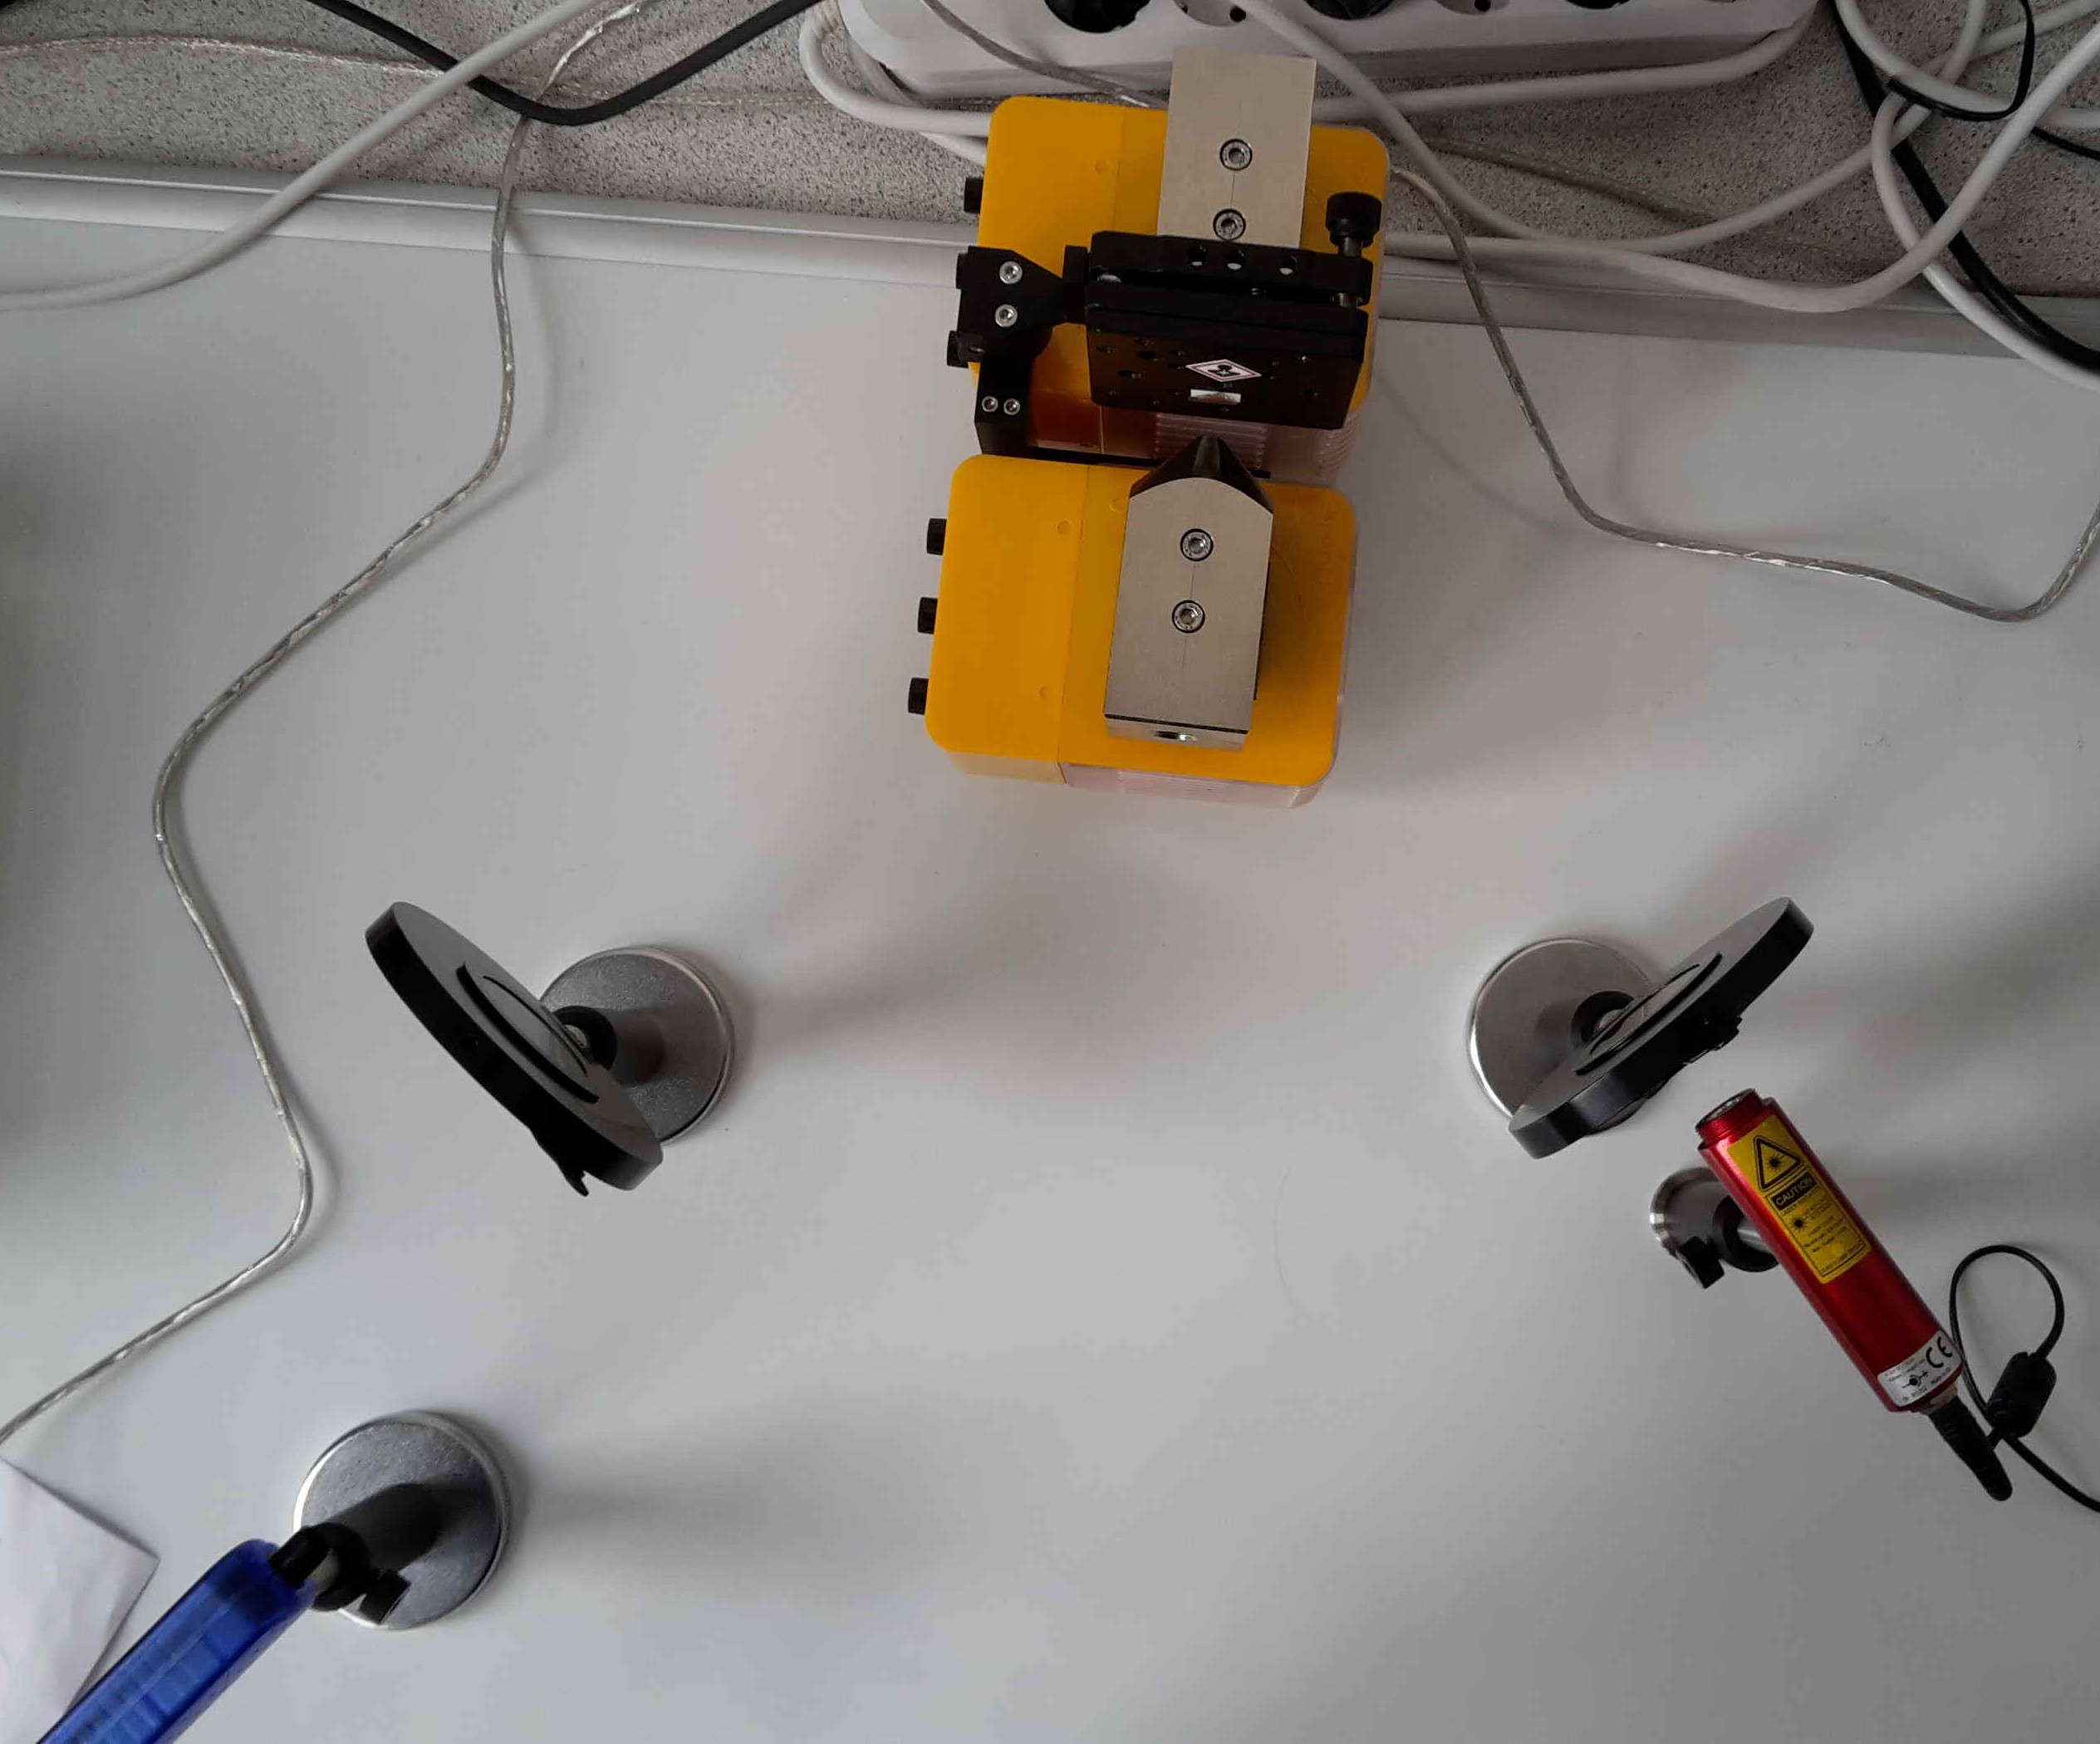
\includegraphics[width=0.7\textwidth]{O4_Aufbau}
		\centering
		\caption{Elemente des Aufbaus des Experiments. Ein linear polarisierter Laserstrahl trifft auf eine Probe aus einem Cobalt/Platin-Schichtsystem, die sich in einem Magnetfeld befindet. Der reflektierte Strahl trifft durch einen Polarisationsfilter in einen Lichtsensor. Aus Übersichtsgründen sind keine Kabel angeschlossen. Die optischen Komponenten sind nicht justiert.} 
		\label{fig_aufbau}
		\centering
	\end{figure}
	
	\section{Ergebnisse und Diskussion}
	%TODO Unsicherheiten
	

	\subsection{Beobachtung}
	%TODO Einflüsse von veränderten Parametern auf Messung
	\subsubsection{Unsicherheiten} %TODO GGF IN DATENANYLSY
	\subsection{Datenanalyse}
	%TODO Berechung nach Aufgabenstellung
	
	\subsection{Diskussion}
	%TODO Bezug/Nutzen oder sonst was
	%TODO auch hier die Hypothese wiederholen
	%TODO keine Messwerte hier, nach manchen Menschen, zumindest "direkt" erstellte Diagramme net hier, auch wenn Lesbarkeit-bla
	
	\section{Schlussfolgerung}
	%TODO Rückgriff auf Hypothese und drittes Nennen dieser
	
	%TODO Quellen zitieren, Websiten mit Zugriffsdatum
	%TODO Verweise auf das Laborbuch (sind erlaubt)
	%TODO Tabelle + Bilder mit Beschriftung
	%\printbibliography
\end{document}
